

\tikzset{every picture/.style={line width=0.75pt}} %set default line width to 0.75pt        

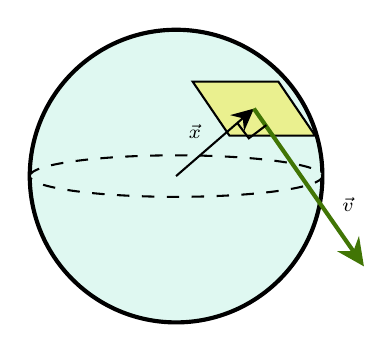
\begin{tikzpicture}[x=0.75pt,y=0.75pt,yscale=-1,xscale=1]
%uncomment if require: \path (0,300); %set diagram left start at 0, and has height of 300

%Shape: Circle [id:dp254606372765645] 
\draw  [fill={rgb, 255:red, 223; green, 248; blue, 241 }  ,fill opacity=1 ][line width=1.5]  (161,152.5) .. controls (161,113.56) and (192.56,82) .. (231.5,82) .. controls (270.44,82) and (302,113.56) .. (302,152.5) .. controls (302,191.44) and (270.44,223) .. (231.5,223) .. controls (192.56,223) and (161,191.44) .. (161,152.5) -- cycle ;
%Shape: Ellipse [id:dp7341918406156717] 
\draw  [fill={rgb, 255:red, 223; green, 248; blue, 241 }  ,fill opacity=1 ][dash pattern={on 4.5pt off 4.5pt}] (161,152.5) .. controls (161,146.98) and (192.56,142.5) .. (231.5,142.5) .. controls (270.44,142.5) and (302,146.98) .. (302,152.5) .. controls (302,158.02) and (270.44,162.5) .. (231.5,162.5) .. controls (192.56,162.5) and (161,158.02) .. (161,152.5) -- cycle ;
%Shape: Parallelogram [id:dp1888887727044548] 
\draw  [fill={rgb, 255:red, 248; green, 231; blue, 28 }  ,fill opacity=0.46 ] (280.8,107) -- (239.5,107) -- (257.2,133) -- (298.5,133) -- cycle ;
%Straight Lines [id:da5934768392694703] 
\draw    (231.5,152.5) -- (266.73,121.96) ;
\draw [shift={(269,120)}, rotate = 139.09] [fill={rgb, 255:red, 0; green, 0; blue, 0 }  ][line width=0.08]  [draw opacity=0] (10.72,-5.15) -- (0,0) -- (10.72,5.15) -- (7.12,0) -- cycle    ;
%Straight Lines [id:da12457450880261867] 
\draw [color={rgb, 255:red, 65; green, 117; blue, 5 }  ,draw opacity=1 ][line width=1.5]    (269,120) -- (319.71,192.72) ;
\draw [shift={(322,196)}, rotate = 235.11] [fill={rgb, 255:red, 65; green, 117; blue, 5 }  ,fill opacity=1 ][line width=0.08]  [draw opacity=0] (13.4,-6.43) -- (0,0) -- (13.4,6.44) -- (8.9,0) -- cycle    ;
%Shape: Right Angle [id:dp8028801232030925] 
\draw   (275,127.95) -- (266.56,134.3) -- (261.02,126.94) ;

% Text Node
\draw (236,126.4) node [anchor=north west][inner sep=0.75pt]  [font=\scriptsize]  {$\vec{x}$};
% Text Node
\draw (310,161.4) node [anchor=north west][inner sep=0.75pt]  [font=\scriptsize]  {$\vec{v}$};


\end{tikzpicture}
